% !TEX root = owasp-doc.tex

% ================================================
%	LLM Strategy
% ================================================

\headerimage

\chapter{Determining LLM Strategy}

The acceleration of LLM applications has raised the visibility of all
artificial intelligence applications' organizational use. Recommendations for
policy, governance, and accountability should be considered holistically.

The immediate LLM threats are the use of online tools, browser plugins,
third-party applications, the extended attack surface, and ways attackers can
leverage LLM tools to facilitate attacks.

\begin{figure}[h]
  \centering
  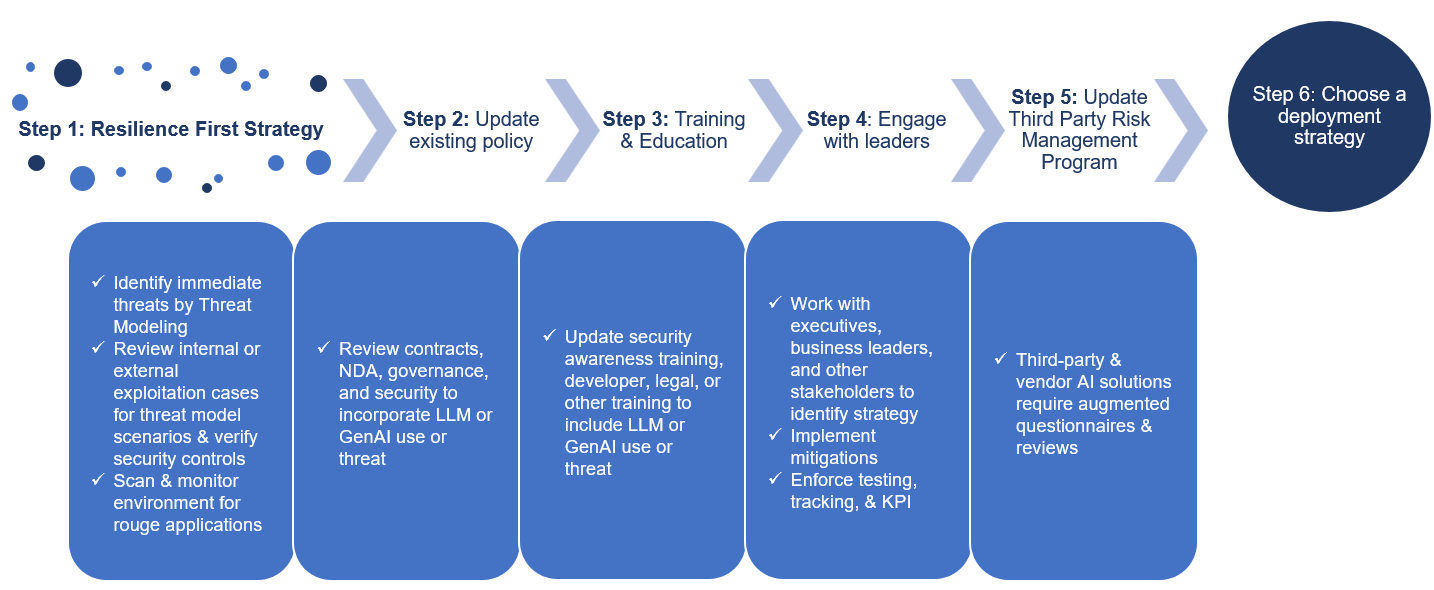
\includegraphics[width=\textwidth]{ai_implementation_strategy}
  \caption{Image of steps of LLM implementation}
  \label{fig:llm-implementation-strategy}
\end{figure}

\clearpage

\section{Deployment Strategy}

The scopes range from leveraging public consumer applications to training
proprietary models on private data. Factors like use case sensitivity,
capabilities needed, and resources available help determine the right balance
of convenience vs. control. But understanding these five model types provides a
framework for evaluating options.

\begin{figure}[h]
  \centering
  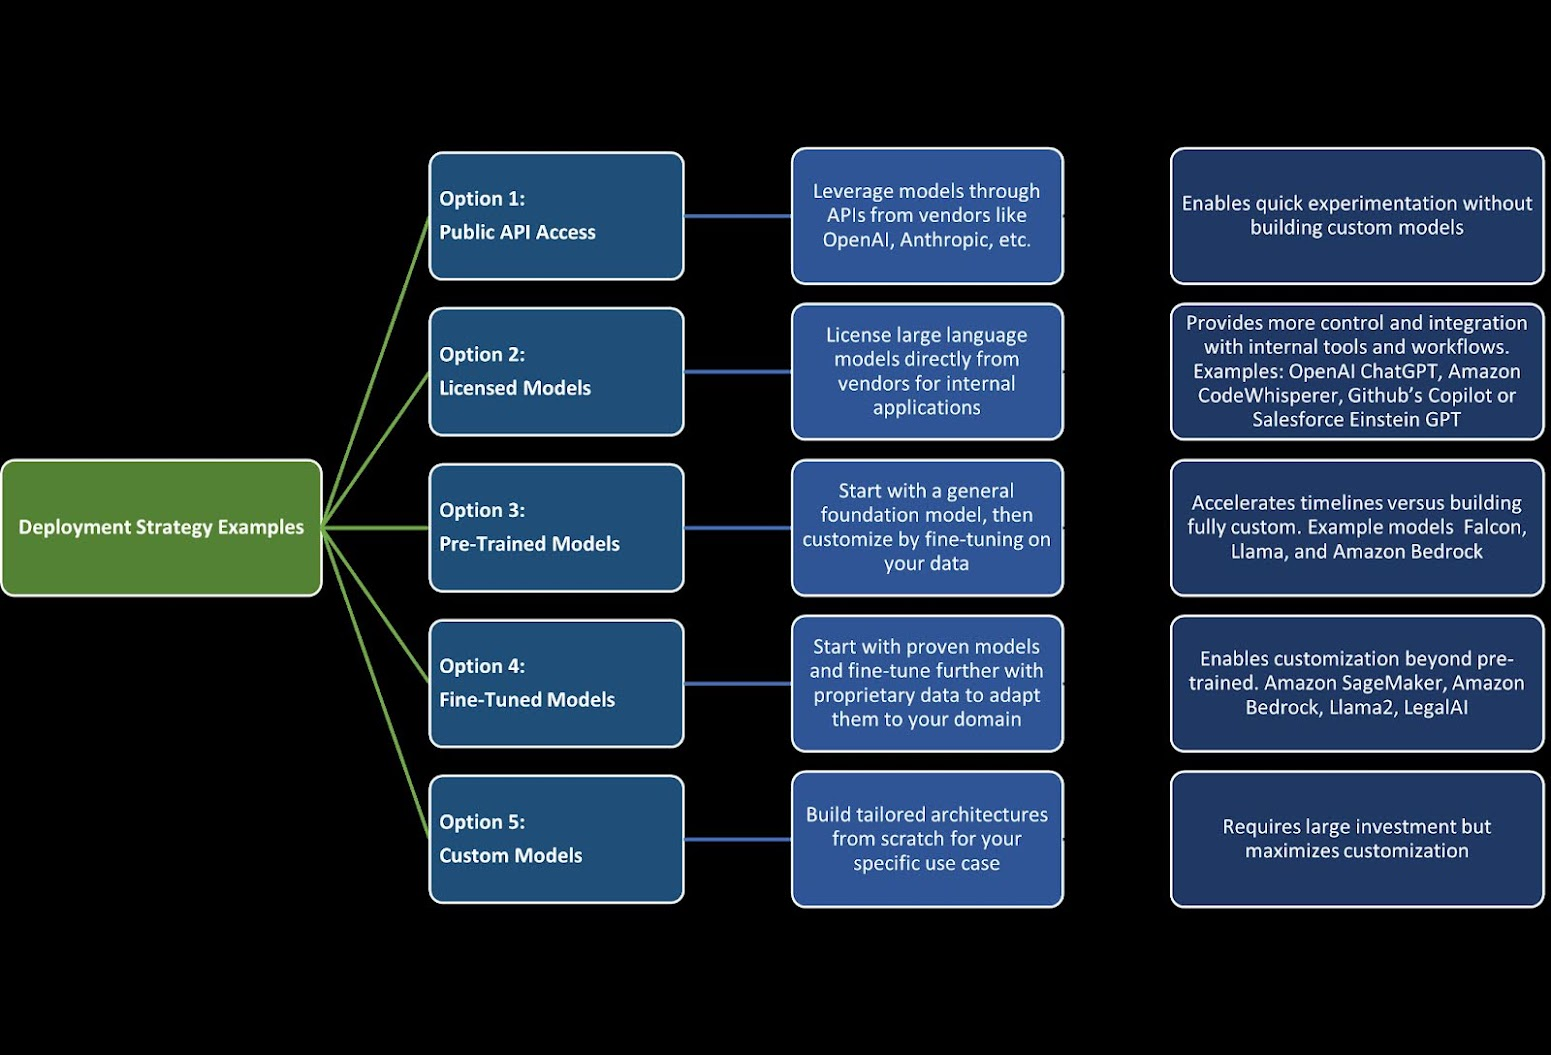
\includegraphics[width=\textwidth]{ai_deployment_strategy}
  \caption{Image of options for deployment strategy}
  \label{fig:llm-deployment-strategy}
\end{figure}
